\chapter{Aprendizado de regras}

\section{Autômato celular}

Os modelos de autômatos celulares foram testados primeiramente, e até o momento, apenas no conjunto de proteínas com alta identidade sequencial. A escolha desse conjunto para os testes dos autômatos celulares baseou-se na facilidade de observar e analisar a formação e propagação dos elementos de estruturas secundárias nessas proteínas.

O modelo idealizado para o autômato celular deveria ter a capacidade de propagar sinais locais ao longo da sequência, e assim, resultar na formação de padrões globais. Tal capacidade está relacionada aos estados que ocorrem durante a evolução do autômato celular, sendo dependentes do número de estados possíveis e também do tamanho da vizinhança utilizada. Como todos os autômatos celulares propostos tem vizinhança 1 por questões de complexidade (ver ref metodos), a capacidade de formar e propagar os sinais será dependente apenas dos estados possíveis do autômato celular.

Entre os quatro modelos testados, o número de estados para os elementos de estrutura secundária demonstrou relação com a acurácia do modelo. Assim, CAs com estados de elementos de estrutura secundária que mantém mais características dos resíduos mostraram-se mais promissores (Figura \ref{fig:ca_errors}).

\begin{figure}
  \centering
  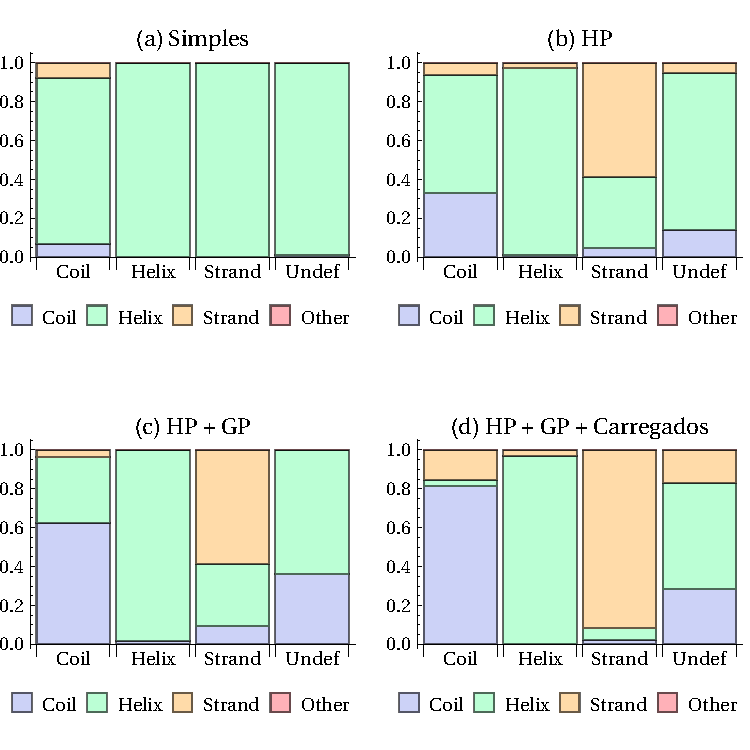
\includegraphics[width=.9\textwidth]{figures/chamel_errors_ca.pdf}
  \caption{Figura da sequencia e das estruturas das camaleonicas}
        \label{fig:ca_errors}
\end{figure}

\begin{figure}
  \centering
  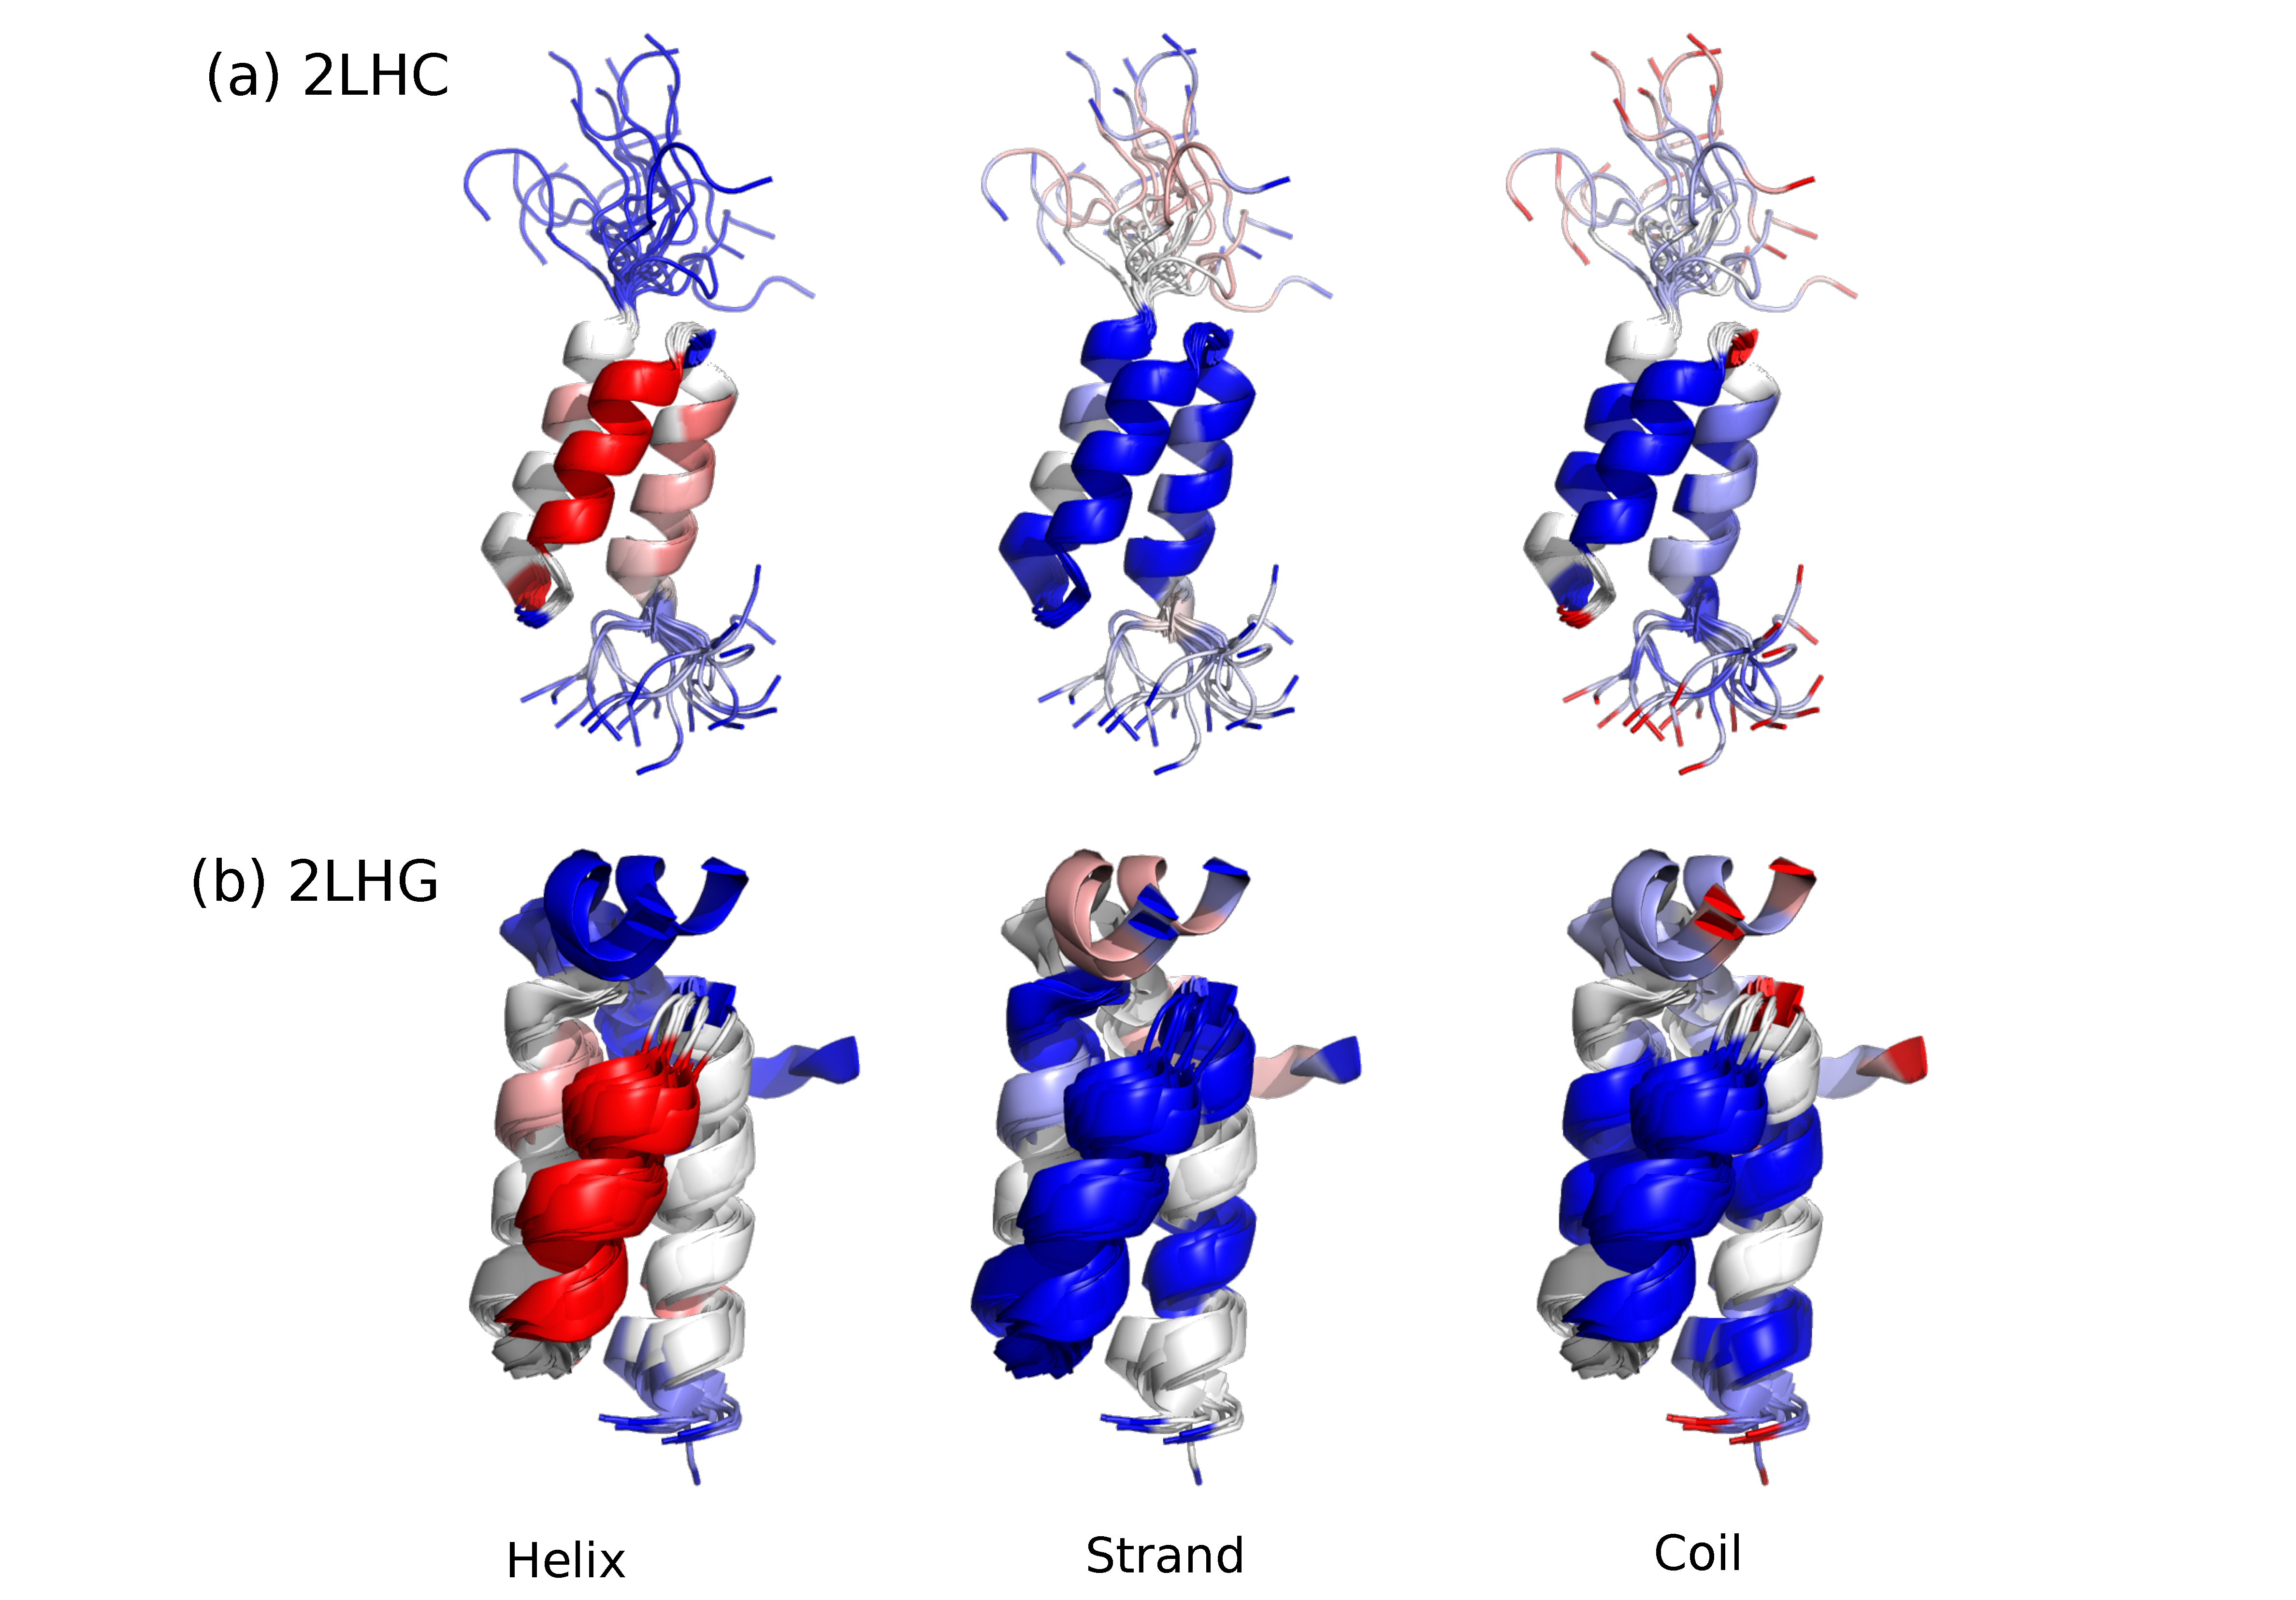
\includegraphics[width=1\textwidth]{figures/camel_2lhc_2lhg.pdf}
  \caption{Figura da sequencia e das estruturas das camaleonicas}
        \label{fig:camel_2lhc_2lhg}
\end{figure}

\begin{figure}
  \centering
  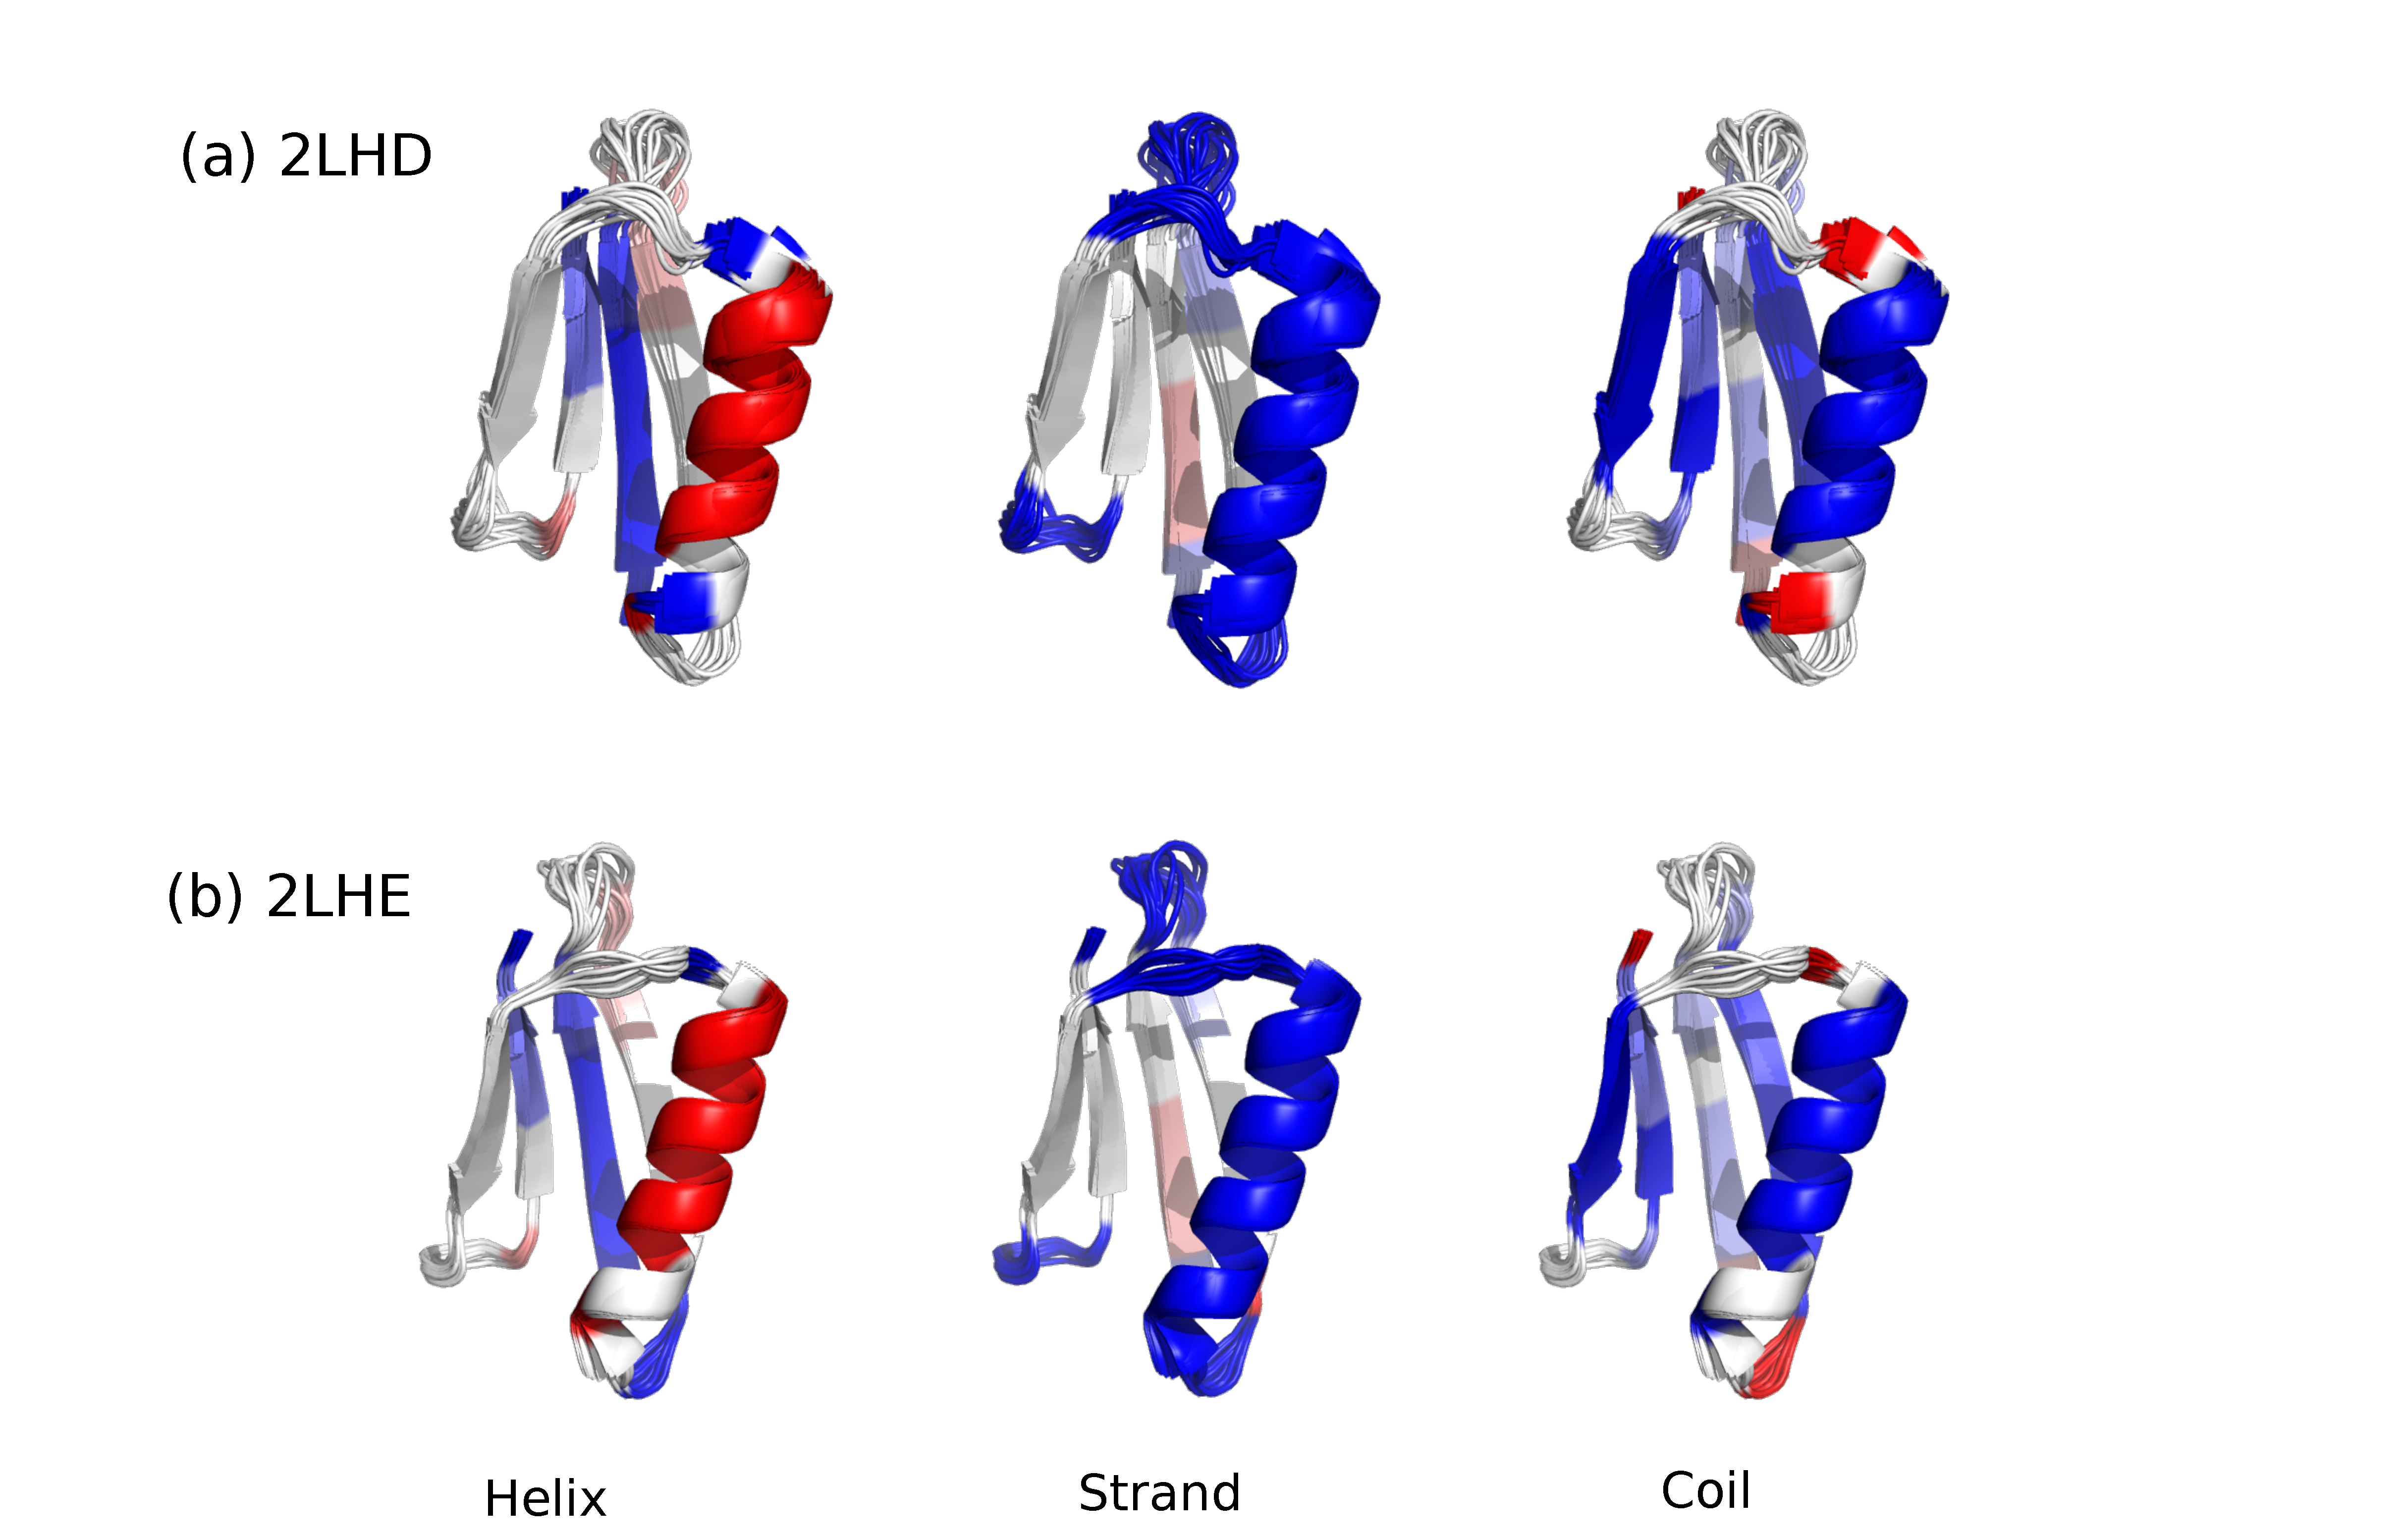
\includegraphics[width=1\textwidth]{figures/camel_2lhd_2lhe.pdf}
  \caption{Figura da sequencia e das estruturas das camaleonicas}
        \label{fig:camel_2lhd_2lhe}
\end{figure}




\section{EDA}

O aprendizado das regras realizado através de um algoritmo de EDA distribuído demonstrou-se eficiente dado a complexidade do problema. Utilizando ?? nós (??CPUs) no cluster multiusuário da FAPESP localizado em ??? São Paulo foi possível evoluir o EDA por 1000 com 10000 indivíduos em pouco mais de duas semanas (CONFIRMAR ISSO).

Cada nó de trabalho apresentou um uso de memória de XX\% (MB), e manteve o processamento próximo a XX\% por núcleo (1.6 GHz). O mecanismo de comunicação por RPC entre o nó mestre e os nós de trabalho não sobrecarregou a rede (1Gbs). Isso nos permite concluir que o algoritmo é escalável clusters com maior número de nós e processadores de maior desempenho.

A opção por realizar o torneio entre soluções candidatas nos nós de trabalho, permite apenas a opção de realizar o torneio entre a k últimas soluções geradas no próprio nó. Consequentemente, as k-1 soluções perdedoras são descartadas, portanto, há a remoção das soluções perdedoras em cada torneio. Comumente, o método de seleção por torneio utilizado em algoritmos genéticos não distribuídos acumula as solução candidatas até atingir o tamanho máximo populacional, quando então, é realizado o torneio. Isso permite que o torneio seja feito sem a eliminação dos perdedores, possibilitando que a seleção destes ocorram em outros combates.

Entretanto, no EDA distribuído seria necessário:
1- o envio de todas as soluções candidatas para o nó mestre, o que resultaria em maior consumo de rede.
2- o acúmulo de todas as soluções candidatas até atingir o tamanho máximo da população, gerando uma limitação da memória disponível.
3- a espera até a realização do torneio para iniciar o cálculo das probabilidades, resultando aumento do tempo de ociosidade nos nós igual ao intervalo de tempo do envio da última solução até o cálculo das probabilidades. 

A escolha em realizar o torneio nos nós de trabalho demonstrou ser mais escalável, mantendo a valiabilidade das soluções candidatas ao longo da evolução e boa convergência (Figura de convergência e variabilidade).

A evolução do EDA por 1000 gerações, mesmo com uma população de 10000 indivíduos, não apresentou sinais de deriva genética com torneio de dois indivíduos (k=2) como podemos notar pelas probabilidades de 20 regras ausentes do conjunto de treinamento. Não foram testados torneios com maior número de indivíduos uma vez que a convergência ocorreu após apenas ??? gerações.  

     
correlacao freq regras x convergencia
correlacao freq de ss regras x convergencia
plot 3D freq regras x freq ss x convergencia


A simplicidade da equação de fitness (referencia a equaçao) demonstrou problemas que acreditamos serem solucionáveis na continuação do desenvolvimento deste trabalho. Um desses problemas é ocasionado pelo desbalanceamento dos dados de treinamento (Figura distribuição). 

Os resultados obtidos indicam uma maior acurácia para os elementos de estrutura secundária mais frequentes no conjunto de treinamento. Esse é um problema recorrente no aprendizado com classes desbalanceadas e costuma ser tratado na função de fitness (figura q3). 

Avaliamos também se havia alguma relação aparente dos elementos preditos com os ângulos phi e psi do resíduos, o que poderia justificar parcilamente o erro nos elementos preditos. Entretanto, aparentemente não existe tal relação (figuras).

Outra modificação possível na função de fitness seria buscar a maximização da frequência dos estados durante a evolução do autômato.  
























A proteína Ga98 e seus mutantes, os quais sofrem alterações globais na estrutura secundária, são casos interessantes para o teste de novas metodologias de predição de estrutura secundária. Nas metodologias atuais, que comumente utilizam redes neurais, a predição é feita utilizando uma janela de resíduos, em geral com comprimentos de 9, 11 ou 13 resíduos, onde o resíduo central da janela é classificado pela rede neural. Como a predição nas demais janelas presentes na sequência polipeptídica não influencia na classificação da janela, o método apresenta a limitação de responder apenas localmente às variações dos dados de entrada.  

Por outro lado, os autômatos celulares, apesar de evoluirem de acordo com regras locais, tem a capacidade de propagar as variações locais e influenciar o surgimento ou alteração de padrões globais, distantes do ponto de origem da variação. 

Para avaliar a capacidade dos modelos propostos e da eficácia do método de otimização em encontrar regras capazes de reproduzir o padrão correspondente às estruturas secundárias, testamos a nossa metodologia nessas quatro proteínas.



\chapter{Aprendizado das regras gerais}




\section{contagem de aa}
CCW      2
CMW      2
WMC      2
WPC      3
WCW      3
CHW      4
MWC      4
CCC      4
CMC      4
WCC      4
CWW      4
WWM      5
MCW      5
CWC      5
MWM      6
CCM      6
MWH      6
CWH      6
FWC      6
QCC      6
QCW      6
WWW      6
WCH      7
CMM      7
YCW      7
WCM      7
CIW      7
HWC      7
CQW      7
CYW      8
..     ...
AAE   1000
LKE   1001
AEA   1011
EAA   1021
AGA   1029
AGL   1032
AAV   1034
AEL   1046
ELA   1051
EEL   1066
ALG   1076
LGL   1080
LAG   1082
VAA   1105
ALE   1111
LEA   1111
AVA   1118
ELL   1129
LAL   1131
LLE   1166
LAE   1172
AAG   1246
ALL   1289
LLA   1296
EAL   1316
LAA   1478
AAL   1534
ALA   1563
AAA   1682
HHH   6143